\section{Implementación}
%=====================================================================
\subsection{Lectura de registros WFDB}
El flujo de carga es: cabecera $\rightarrow$ validación $\rightarrow$ decodificación por archivo $\rightarrow$ conversión de unidades $\rightarrow$ \texttt{RegistroECG}. El analizador de cabeceras interpreta cada línea de señal con expresiones regulares para el formato (\texttt{formato[xN][:skew][+offset]}) y la ganancia (\texttt{ganancia[(baseline)][/unidades]}); si no hay línea base explícita se adopta el valor ADC cero. Los registros multisegmento se rechazan con un mensaje explícito.

Las señales se agrupan por archivo y cada grupo se decodifica con la implementación correspondiente a su formato. El formato 16 son enteros de 16 bits con signo \emph{little-endian}. En el formato 212, dos muestras de 12 bits comparten tres bytes; numerando las muestras intercaladas con $k=0,1,\dots$ y siendo $b$ el desplazamiento del grupo de tres bytes $(b_0,b_1,b_2)$ al que pertenece:
\begin{equation}
v_k=\begin{cases}
b_0+256\,(b_1\ \&\ \mathrm{0x0F}) & k\ \text{par},\\
b_2+16\,(b_1\ \&\ \mathrm{0xF0}) & k\ \text{impar},
\end{cases}
\end{equation}
con extensión de signo de 12 bits. En el formato 8 se acumulan diferencias con signo a partir del valor inicial de cada señal; los formatos 24 y 32 son enteros de 3 y 4 bytes. Este diseño por intercalado global permite cualquier número de canales, incluido un número impar con muestra final a medias.

La conversión \eqref{eq:conv} se realiza en una única clase. Las unidades de tensión se normalizan a mV ($\mu$V, V, nV); las no eléctricas se conservan. El valor reservado $-32768$ del formato 16 se transforma en \texttt{NaN} (muestra inválida), que el renderizador representa como un hueco. Un registro sin ganancia declarada se rechaza en lugar de aplicar un valor supuesto. Finalmente, la suma módulo $2^{16}$ de cada señal se compara con el \emph{checksum} de la cabecera para detectar errores de decodificación; una discrepancia genera una advertencia, pero no bloquea la carga.


\subsection{Procesamiento de señal}

El procesamiento se organiza en dos etapas encadenadas sobre cada derivación $x[n]$ de frecuencia $f_s$: (i) \textbf{detección de complejos QRS} y (ii) \textbf{clasificación de cada latido} en una de las cuatro clases AAMI (N, S, V, F) mediante un \emph{Random Forest}. Todo el cómputo es independiente de $f_s$: las ventanas se definen en segundos y se convierten a muestras con $\lfloor w f_s \rceil$.

\subsubsection{Detección QRS (Pan-Tompkins con media móvil)}

El detector procesa cada derivación con ventanas definidas en segundos:
\begin{align}
y_1[n]&=x[n]-\mathrm{MM}_{0{,}20 f_s}(x)[n],\quad y_2=\mathrm{MM}_{0{,}025 f_s}(y_1),\\
d[n]&=\tfrac{1}{8}\bigl(2y_2[n{+}2]+y_2[n{+}1]-y_2[n{-}1]-2y_2[n{-}2]\bigr),\\
m&=\mathrm{MM}_{0{,}15 f_s}\!\bigl(d^{2}\bigr),
\end{align}
donde $\mathrm{MM}_w$ es una media móvil centrada de $w$ muestras calculada en $O(n)$ con sumas acumuladas. Sobre $m$ se buscan máximos locales y se mantienen las estimaciones de nivel de señal ($S$) y de ruido ($N$) con
\begin{align}
S&\leftarrow \tfrac18 m_i+\tfrac78 S,\qquad N\leftarrow \tfrac18 m_i+\tfrac78 N,\\
\theta&=N+\tfrac14(S-N).
\end{align}
Un candidato se acepta si $m_i>\theta$ y han pasado más de 0,2\,s desde el latido previo (periodo refractario); si cae a menos de 0,36\,s del previo y su pendiente máxima $|d|$ es menor que la mitad de la del latido previo, se trata como onda T. El pico se refina al máximo de $|y_2|$ en $\pm 0{,}08$\,s, lo que permite detectar R negativas (p.~ej. aVR). La pendiente máxima en ventana se calcula en $O(n)$ con un \emph{deque} monótono (\texttt{maxAbsVentana}), evitando el coste $O(n\cdot w)$ del cálculo ingenuo. No se implementó la búsqueda hacia atrás de latidos perdidos.

\subsubsection{Fusión de canales por consenso}

El detector se ejecuta por derivación y los resultados se combinan por consenso (Alg.~\ref{alg:fusion}): los candidatos de todos los canales se ordenan, se agrupan cuando la distancia entre consecutivos es inferior a 0,1\,s y se aceptan los grupos con al menos $\lceil n/2\rceil$ canales distintos, usando la mediana como posición del latido. A partir de los latidos se calculan los intervalos $RR_i=(n_{i+1}-n_i)/f_s$, la frecuencia instantánea $FC_i=60/RR_i$ y las medidas SDNN y RMSSD.

\begin{algorithm}[t]
\small
\caption{Fusión de detecciones por consenso}
\label{alg:fusion}
\begin{algorithmic}[1]
\Require detecciones por canal, ventana $w$, votos mínimos $v$
\Ensure lista de latidos fusionados
\State $C\leftarrow$ todos los pares (índice, canal), ordenados por índice
\State $g\leftarrow\emptyset$
\ForAll{$c\in C$}
  \If{$g\neq\emptyset$ \textbf{y} $c.\mathrm{indice}-\mathrm{ultimo}(g).\mathrm{indice}>w f_s$}
    \State cerrar($g$); $g\leftarrow\emptyset$
  \EndIf
  \State añadir $c$ a $g$
\EndFor
\State cerrar($g$) \Comment{acepta si canales distintos $\ge v$; guarda la mediana}
\end{algorithmic}
\end{algorithm}

\subsubsection{Extracción de características por latido}

Cada latido detectado en la posición $p$ se describe con \textbf{257 números} (vector de características $\phi\in\mathbb{R}^{257}$), calculados por \texttt{Caracteristicas.extraer}:

\textbf{Forma del latido (252 valores).} Sea $c=\mathrm{recentrar}(x,p)$ el pico R refinado al mayor $|x-\mathrm{mediana}|$ en $\pm 50$\,ms. La ventana de forma es
\begin{equation}
f_j \;=\; x[c-90+j]-\tilde{x},\qquad j=0,\dots,251,
\end{equation}
donde $\tilde{x}$ es la mediana de $x$ en $[c-90,\,c+162)$ y se usan 90 muestras antes y 162 desde el pico (a 360\,Hz: 0,25\,s y 0,45\,s). Restar la mediana elimina la línea base.

\textbf{Ritmo (5 valores).} Con $d_i=c_i-c_{i-1}$ el número de muestras entre latidos consecutivos y $\overline{d}_i$ la media de los últimos 10 $d$:
\begin{equation}
\phi_{252..256}=\Bigl(\tfrac{d_{i-1}}{f_s},\;\tfrac{d_{i+1}}{f_s},\;\tfrac{\overline{d}_i}{f_s},\;\tfrac{d_{i-1}}{\overline{d}_i},\;\tfrac{d_{i+1}}{\overline{d}_i}\Bigr).
\end{equation}
Estos cinco valores capturan latidos que llegan antes o después de lo normal (extrasístoles, pausas). Si la ventana de 252 muestras no cabe en la señal (extremos del registro), el latido se descarta para clasificación pero \textbf{sí} cuenta para los intervalos RR.

\subsubsection{Clasificación con Random Forest}

El clasificador es un \textbf{Random Forest de $T$ árboles de decisión} implementado sin librerías externas (\texttt{BosqueSimple}, \texttt{ArbolDesicion}). Cada árbol $t$ se entrena con un \textbf{bootstrap} de las muestras de DS1 (filas sorteadas con repetición) y, en cada nodo, considera solo un subconjunto aleatorio de $k=\lfloor\sqrt{257}\rfloor\approx 16$ características.

\textbf{Criterio de corte.} En un nodo con muestras $\mathcal{S}$, la \textbf{entropía de Shannon} de las clases es
\begin{equation}
H(\mathcal{S})=-\sum_{c=1}^{4} p_c\log_2 p_c,\qquad p_c=\frac{|\{m\in\mathcal{S}:y_m=c\}|}{|\mathcal{S}|},
\end{equation}
y la \textbf{ganancia de información} de un corte ``$\phi_j<\theta$'' es
\begin{equation}
\Delta H(\mathcal{S},j,\theta)=H(\mathcal{S})-\frac{|\mathcal{S}_{\mathrm{izq}}|}{|\mathcal{S}|}H(\mathcal{S}_{\mathrm{izq}})-\frac{|\mathcal{S}_{\mathrm{der}}|}{|\mathcal{S}|}H(\mathcal{S}_{\mathrm{der}}).
\end{equation}
Para cada característica candidata $j$ se fija $\theta=\overline{\phi_j}$ (la media de esa característica en el nodo) y se elige el par $(j^\star,\theta^\star)$ de mayor $\Delta H$. El nodo se parte en $\mathcal{S}_{\mathrm{izq}}=\{m:\phi_{m,j^\star}<\theta^\star\}$ y $\mathcal{S}_{\mathrm{der}}$ el resto, y se repite recursivamente hasta que el grupo es puro, tiene menos de $\ell_{\min}$ muestras, o ninguna partición lo separa. Cada hoja guarda la \textbf{distribución empírica de clases} $p=(p_N,p_S,p_V,p_F)$ de sus muestras.

\textbf{Predicción (voto blando).} Para un latido nuevo con vector $\phi$, cada árbol $t$ devuelve la distribución $p^{(t)}(\phi)$ de la hoja alcanzada. El bosque promedia:
\begin{equation}
\hat{p}(\phi)=\frac{1}{T}\sum_{t=1}^{T}p^{(t)}(\phi),\qquad \hat{y}=\arg\max_{c\in\{N,S,V,F\}}\hat{p}_c(\phi).
\end{equation}
La doble aleatoriedad (bootstrap de filas + subconjunto de características por nodo) descorrelaciona los árboles y reduce la varianza del ensamble frente a un árbol único. Con semilla fija el bosque es reproducible bit a bit.

\textbf{Fusión entre derivaciones.} Si el registro tiene varias derivaciones, cada latido se clasifica en todas ellas (cuando la ventana cabe) y se promedian las distribuciones $\hat{p}^{(d)}$ de las derivaciones votantes antes de aplicar el $\arg\max$; si solo una derivación aporta, se usa directamente.

\begin{algorithm}[t]
\small
\caption{Entrenamiento de un árbol del bosque (nodo $\mathcal{S}$)}
\label{alg:arbol}
\begin{algorithmic}[1]
\Require muestras $\mathcal{S}$, nº clases $C{=}4$, características por nodo $k$, mínimo de hoja $\ell_{\min}$
\Ensure nodo del árbol
\If{$|\mathcal{S}|<\ell_{\min}$ \textbf{o} todas las $y_m$ iguales}
  \State \Return hoja con distribución $p_c=|\{m:y_m=c\}|/|\mathcal{S}|$
\EndIf
\State $\mathcal{J}\leftarrow$ subconjunto aleatorio de $k$ características
\State $(j^\star,\theta^\star)\leftarrow\arg\max_{j\in\mathcal{J},\,\theta=\overline{\phi_j}}\Delta H(\mathcal{S},j,\theta)$
\State partir $\mathcal{S}$ en $\mathcal{S}_{\mathrm{izq}},\mathcal{S}_{\mathrm{der}}$ por $(j^\star,\theta^\star)$
\If{$\mathcal{S}_{\mathrm{izq}}=\emptyset$ \textbf{o} $\mathcal{S}_{\mathrm{der}}=\emptyset$}
  \State \Return hoja con distribución de $\mathcal{S}$
\EndIf
\State \Return nodo interno $(j^\star,\theta^\star)$ con hijos
  \textsc{Árbol}$(\mathcal{S}_{\mathrm{izq}})$ y \textsc{Árbol}$(\mathcal{S}_{\mathrm{der}})$
\end{algorithmic}
\end{algorithm}

\subsubsection{Validación de detección y clasificación}

La validación de la \textbf{detección} compara detecciones y referencia con emparejamiento uno a uno y tolerancia $\tau$, calculando verdaderos positivos (TP), falsos positivos (FP) y falsos negativos (FN):
\begin{equation}
Se=\frac{TP}{TP+FN},\quad P^{+}=\frac{TP}{TP+FP},\quad F_1=\frac{2\,Se\,P^{+}}{Se+P^{+}},
\end{equation}
además del error temporal medio $|\Delta t|$ de los latidos emparejados. La validación de la \textbf{clasificación} usa la matriz de confusión $4\times4$ $M[\text{real}][\text{predicho}]$ y, por clase $c$ (uno contra el resto), calcula
\begin{align}
P_c&=\frac{M_{cc}}{\sum_i M_{ic}},\qquad
R_c=\frac{M_{cc}}{\sum_j M_{cj}},\\
F1_c&=\frac{2P_cR_c}{P_c+R_c},\qquad
\text{F1}_{\text{macro}}=\frac14\sum_c F1_c.
\end{align}


\subsubsection{Flujo completo (pipeline)}
\begin{figure}[t]
\centering
\begin{tikzpicture}[
  caja/.style={draw,rounded corners=2pt,minimum height=0.65cm,minimum width=6.3cm,
               font=\scriptsize,align=center,fill=blue!6,inner sep=2pt},
  cajaA/.style={draw,rounded corners=2pt,minimum height=0.65cm,minimum width=6.3cm,
                font=\scriptsize,align=center,fill=green!8,inner sep=2pt},
  cajaB/.style={draw,rounded corners=2pt,minimum height=0.65cm,minimum width=6.3cm,
                font=\scriptsize,align=center,fill=orange!10,inner sep=2pt},
  flecha/.style={-{Stealth[length=1.8mm]},thick},
  etiq/.style={font=\tiny,above,midway,align=center}]

  \node[cajaA] (reg)  {Registro WFDB (\texttt{.hea}/\texttt{.dat}/\texttt{.atr})};
  \node[caja,below=0.20cm of reg]  (det)  {\texttt{DetectorPanTompkins.detectar}$(x_d,f_s)$};
  \node[caja,below=0.20cm of det]  (fus)  {\texttt{FusionDetecciones.fusionar}$(\dots,\lceil n/2\rceil)$};
  \node[caja,below=0.20cm of fus]  (car)  {\texttt{Caracteristicas.extraer}$(x,\text{pos.})$};
  \node[cajaB,below=0.20cm of car] (bos)  {\texttt{BosqueSimple.predecirDistribucion}$(\phi)$};
  \node[caja,below=0.20cm of bos]  (arg)  {$\arg\max_c\,\hat{p}_c(\phi)\;\to$\; AAMI ($N/S/V/F$)};
  \node[cajaA,below=0.20cm of arg] (met)  {\texttt{Metricas.matrizConfusion}\,/\,\texttt{reporte}};

  \draw[flecha] (reg) -- node[etiq] {índices $R$} (det);
  \draw[flecha] (det) -- node[etiq] {latidos} (fus);
  \draw[flecha] (fus) -- node[etiq] {$\phi\in\mathbb{R}^{257}$} (car);
  \draw[flecha] (car) -- node[etiq] {$\hat{p}$} (bos);
  \draw[flecha] (bos) -- node[etiq] {$\hat y$} (arg);
  \draw[flecha] (arg) -- node[etiq] {} (met);
\end{tikzpicture}
\caption{Flujo completo de procesamiento: detección QRS por derivación, fusión por consenso, extracción de las 257 características, clasificación con el bosque aleatorio (voto blando) y validación opcional contra la referencia.}
\label{fig:pipeline}
\end{figure}

\subsubsection{Parámetros e implementación}

\begin{table}[t]
\centering
\footnotesize
\setlength{\tabcolsep}{3pt}
\begin{tabular}{@{}lcc@{}}
\toprule
Parámetro & Valor & Archivo \\
\midrule
Árboles del bosque $T$ & 25 & \texttt{Bosque\-Simple} \\
Caract. por nodo $k$ & $\lfloor\sqrt{257}\rfloor{=}16$ & \texttt{Bosque\-Simple} \\
Mín. de muestras por hoja $\ell_{\min}$ & 20 & \texttt{Arbol\-Desicion} \\
Semilla del azar & 0 & \texttt{Muestreo} \\
Ventana de fusión & 0,10\,s & \texttt{Analizador\-ECG} \\
Tolerancia de validación $\tau$ & 0,15\,s & \texttt{Validador\-Deteccion} \\
\bottomrule
\end{tabular}
\caption{Hiperparámetros del detector y del clasificador.}
\label{tab:parametros}
\end{table}

El dataset de entrenamiento (DS1, 22 registros de MIT-BIH) se construye leyendo los WFDB con \texttt{Datos.construir} y se cachea en texto (\texttt{DSV1}) para no releerlos en cada arranque; el bosque entrenado se serializa en formato \texttt{RFV1} (recorrido en preorden, una línea por nodo) mediante \texttt{BosqueSimple.guardar}/\texttt{cargar}, lo que permite reutilizarlo sin re-entrenar. Las estructuras auxiliares (\texttt{DynamicArray}, \texttt{CircularQueue}, \texttt{MovingMean}, \texttt{MinHeap}) están implementadas a mano en \texttt{ecg.ml.estructuras}, sin depender de las colecciones de \texttt{java.util} para el núcleo del algoritmo.

% =====================================================================
% Referencias sugeridas (añádelas a tu .bib o a la bibliografía)
% =====================================================================


\subsection{Motor de dibujo}
El \texttt{RenderizadorECG} recibe un registro, una \texttt{ConfiguracionVista} y una superficie, sin conocer ventanas ni controles. Cada derivación visible ocupa una celda; la ventana temporal $[t_0,t_1]$ se ajusta al ancho $W$ de la celda y la amplitud se escala con la ganancia vertical $g_v$ (mm/mV) y la resolución $\rho$ (píxeles/mm):
\begin{equation}
x(t)=x_0+\frac{t-t_0}{t_1-t_0}W,\qquad
y(v)=y_c-g_v\,\rho\,v .
\end{equation}
La cuadrícula se dibuja en unidades de tiempo y tensión (0,04\,s y 0,1\,mV por cuadro pequeño; 0,2\,s y 0,5\,mV por cuadro grande) y se omiten los trazos con separación inferior a 3 o 6 píxeles. Cuando hay más de dos muestras por columna de píxeles, la señal se dibuja como envolvente mínimo/máximo, lo que acota el coste de repintado por la anchura de la celda y no por la longitud de la ventana. Las distribuciones (cuadrícula $3\times4$, vertical, individual y automática) se calculan con reparto entero para evitar huecos.

La impresión estándar calcula el tamaño de la imagen para que la calibración sea exacta: el ancho de cada celda es $T\cdot 25\cdot\rho$ píxeles para una ventana de $T$ segundos, y su alto $40\,\rho$ ($\pm2$\,mV a 10\,mm/mV). El visor interactivo traduce eventos de ratón y teclado (rueda: zoom horizontal con el instante bajo el cursor fijo; Ctrl+rueda: zoom vertical; arrastre: desplazamiento; Mayús+arrastre: selección de intervalo) en cambios sobre la configuración, tras lo cual repinta.

\begin{figure}[h!]
\centering
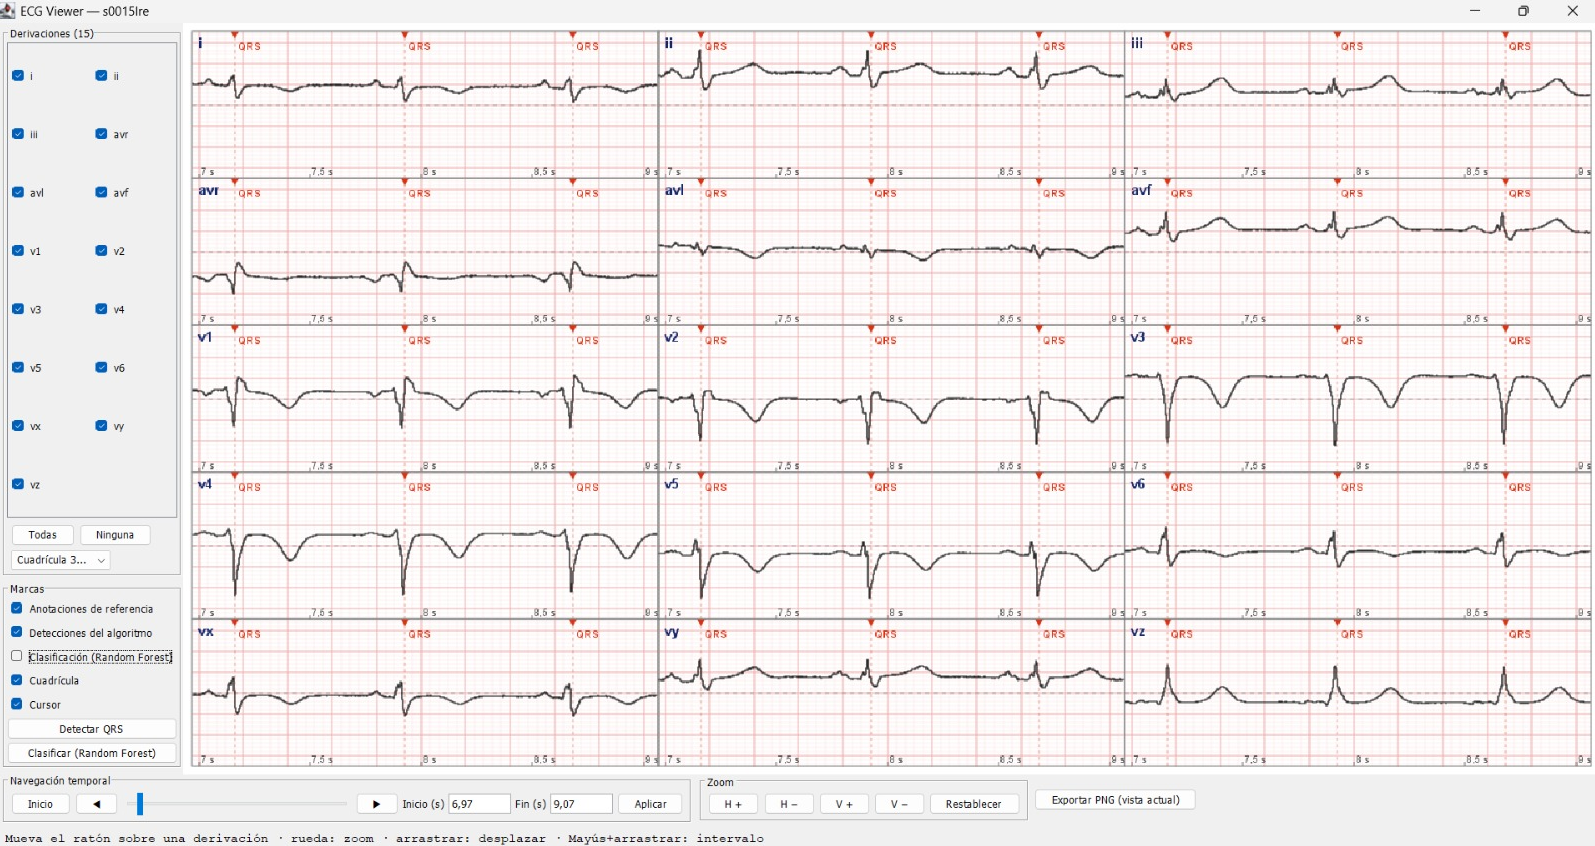
\includegraphics[width=0.44\textwidth]{images/estandar.png}
\caption{Impresión estándar de un registro de la base de datos de PTB Diagnostic ECG Database de 15 derivaciones (distribución $3\times4$, 5\,s, 25\,mm/s y 10\,mm/mV) con detección QRS (triángulos rojos). Imagen generada por la propia aplicación.}
\label{fig:estandar}
\end{figure}

\subsection{Exportación}
Todas las exportaciones heredan de una clase base que dibuja con el mismo \texttt{RenderizadorECG}. Se ofrecen cuatro variantes: impresión estándar, personalizada (derivaciones, intervalo, tamaño, escalas y anotaciones), vista actual (copia de la configuración vigente) y registro completo dividido en páginas de duración fija, para no comprimir registros largos en una sola imagen. Las copias de configuración eliminan el estado de inspección (cursor, selección) para que no aparezca en las impresiones, y se rechazan imágenes de más de $1{,}2\times10^{8}$ píxeles.

\subsection{Medición de rendimiento}
\label{sec:rend}
El \texttt{MonitorRendimiento} inicia una medición antes de cada operación y la cierra después, también si la operación falla; admite operaciones anidadas, registrando su profundidad para no sumar dos veces su coste en los totales. Cada medición combina tres medidores:
\begin{itemize}
  \item \textbf{Tiempo:} diferencia de \texttt{System.nanoTime()}; es tiempo de pared y por tanto incluye esperas.
  \item \textbf{Memoria:} heap usado al inicio y al final, máximo muestreado cada 5\,ms por un hilo auxiliar (una cota inferior del pico real), memoria reservada por la JVM y, en Linux, la memoria residente (RSS) de \texttt{/proc/self/status}.
  \item \textbf{CPU:} nivel portable (CPU del hilo y CPU total del proceso) y nivel específico del sistema operativo (usuario y sistema del proceso desde \texttt{/proc/self/stat}, suponiendo 100 ticks/s). Las magnitudes no disponibles se marcan como tales y nunca se obtienen restando fuentes de distinto origen.
\end{itemize}
El informe PDF (Apache PDFBox~\cite{pdfbox}) contiene la información de la ejecución, las métricas globales, la tabla por operación (con media, mínimo y máximo si hay repeticiones), tres gráficos generados con Java2D, información de aciertos del Random Forest y un apartado de observaciones con las limitaciones de medida. Se genera bajo demanda y no en cada interacción.
\begin{figure}[h!]
\centering
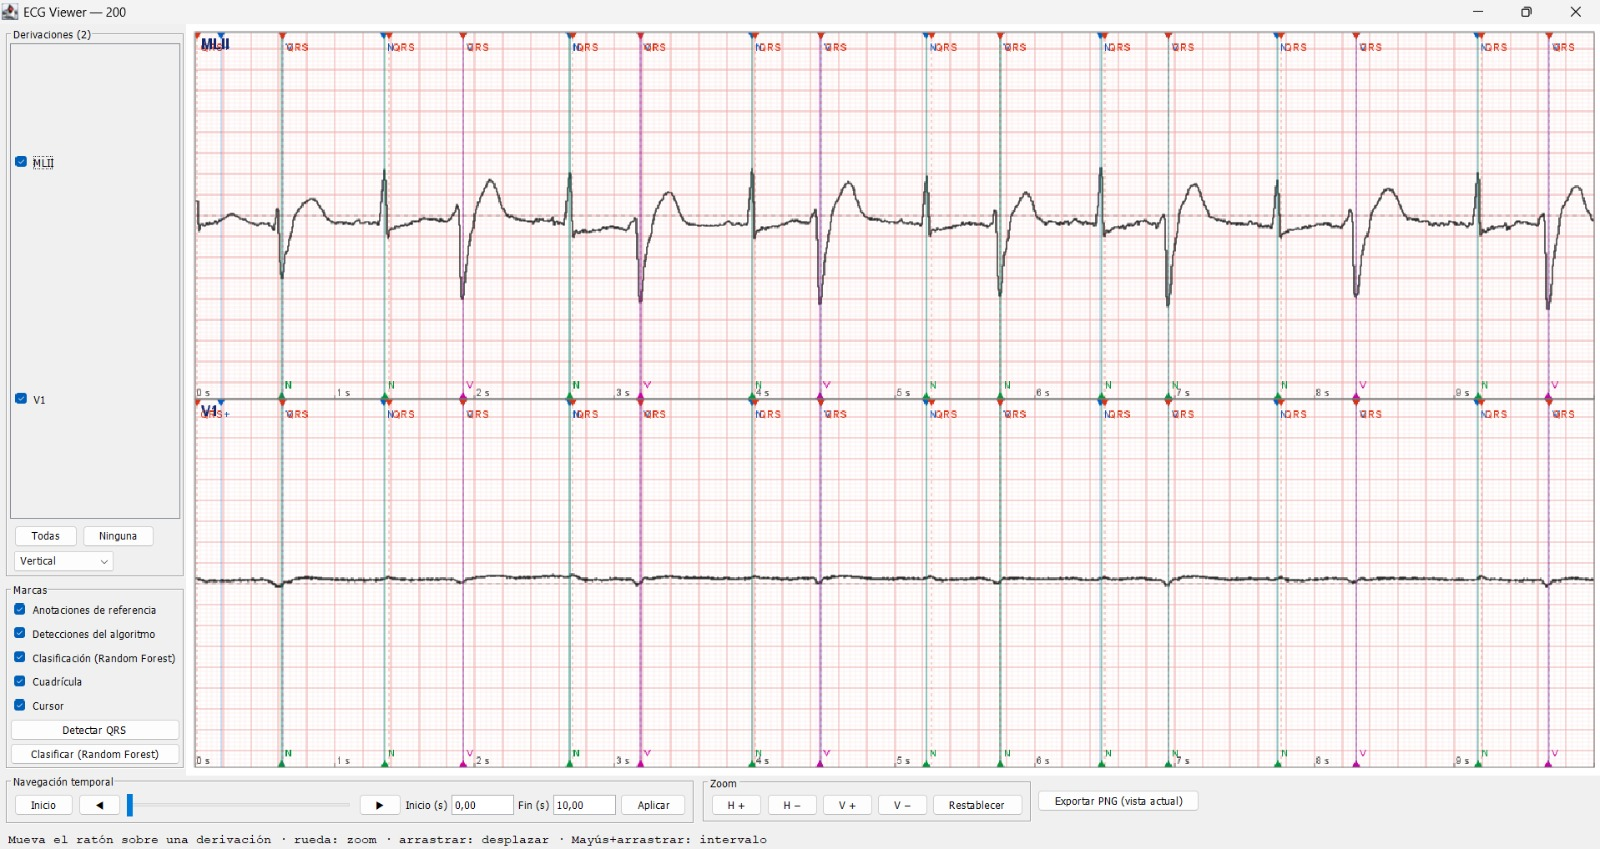
\includegraphics[width=\columnwidth]{images/gui.png}
\caption{Visor interactivo: selección dinámica de derivaciones, controles de distribución, marcas, navegación temporal, zoom y lectura del cursor (tiempo, muestra, derivación y amplitud).}
\label{fig:gui}
\end{figure}



